\documentclass{article}

\usepackage{pdfcomment}
\usepackage[margin=1in]{geometry}
\usepackage{xcolor}
\usepackage{graphicx}
\usepackage{algorithm}
\usepackage{caption}
\usepackage{subcaption}
\usepackage{listings}
\usepackage{verbatim}
\usepackage{booktabs}
\usepackage[flushleft]{threeparttable}


\newcommand{\note}[2]{\pdfmargincomment[color=yellow,author=#1,open=true]{#2}}
\newcommand{\todo}[1]{\color{red}\textbf{TODO:}#1\color{black}}
\newcommand{\reprozip}[0]{ReproZip}

\title{Numerical error propagation in the HCP structural pre-processing pipelines}

\author{M. Ali Salari, Lalet Scaria, Gregory Kiar, Lindsay B. Lewis,
  Alan C. Evans, Tristan Glatard}

\begin{document}

\maketitle

\abstract{This paper is a reproducibility study of the work in~\cite{glasser2015multi}.}

\section{Introduction}

Operating systems are known to have an effect on the results produced
by neuroimaging pipelines~\cite{Gronenschild2012, Glatard2015},
presumably due to the creation, propagation and amplification of small
numerical errors across the pipelines.  Such errors highlight
numerical instability which is also likely to appear as a result of
other types of small perturbations such as acquisition and parametric
noise. However, the precise causes of
such instabilities and the path along which they propagate in the
pipelines are unclear.  We present a technique to identify the
processes in a pipeline that create numerical errors along the
execution, and we apply this technique to the HCP structural
pre-processing pipelines.


Groenschild \emph{et al.} first identified the effect of operating
systems on Freesurfer
results~\cite{Gronenschild2012}. In~\cite{10.3389/fninf.2015.00012} we
quantified this effect on some of the main neuroimaging pipelines
including several FSL pipelines, CIVET and Freesurfer. In this work we
aim at evaluating this effect on the work in~\cite{glasser2015multi}.
\todo{Link this to Lindsay's HBM 2017 poster and to Redolfi et al.}

The operating system is defined here as a consistent set of software
packages organized in a trusted repository.

The operating system is not the only part of the computational
environment that may hamper reproducibility. The work
in~\cite{diethelm2012limits} mentions reproducibility issues coming
from parallelization.

Notes:
\begin{itemize}
  \item Reproducibility has several other aspects, see, e.g.,
\url{https://medium.com/@lorenaabarba/barba-group-reproducibility-syllabus-e3757ee635cf#.ty3zmgd4k}
 \item James P Turner, speaker in INCF 2016 Track B, is looking at numerical stability on GPUs. And reproducibility.
 \item For an overview of variability accross analysis methods in fMRI, see \url{http://journal.frontiersin.org/article/10.3389/fnins.2012.00149/full}.
 \item For a general overview in fMRI, see \url{http://www.nature.com/nrn/journal/vaop/ncurrent/box/nrn.2016.167_BX3.html}
\end{itemize}

% There is a computational challenge
HCP preprocessing pipelines are both time-consuming and
computationally intensive which might even run for days, depending
upon the type and size of dataset.

Any
user who has access to this application can try to reproduce the
experiments since the data and the application are accessible within
the framework. However, one caveat is that, the neuroimaginng
pipelines might have different results due to differences in computing
platforms on which the images are getting processed
~\cite{10.3389/conf.fninf.2014.18.00076} therefore, the execution
results of the pipelines across different operating systems are
considered to find out the cause of the reproducibility issues using
an interposition techniques for the provenance capture.

\todo{Check everywhere that differences are called error. And define that in the intro.}


\section{Materials and Methods}

\subsection{Data}

We randomly selected 10 subjects from the HCP data release
S500 which are described in table~\ref{table:data}. \todo{ list the subjects.}

\begin{table}[H]\hspace*{-1cm}
\centering
\begin{threeparttable}
\caption{An overview of the HCP data (Humman Connectome DB).}

\begin{tabular}{@{}llllll@{}}
\toprule
Subject & Release & Acquisition & Gender & Age      & Subj\_Type   \\ \midrule
103515  & Q1      & Q02         & F      & 26-30    & type1         \\
105216  & Q3      & Q03         & M      & 26-30    & type4         \\
103414  & Q2      & Q02         & F      & 22-25    & type1         \\
125525  & Q1      & Q01         & F      & 31-35    & type1         \\
142828  & Q1      & Q01         & M      & 31-35    & type1         \\
129533  & Q3      & Q04         & F      & 31-35    & type1         \\
103818  & Q1      & Q01         & F      & 31-35    & type3         \\
133928  & Q2      & Q03         & M      & 26-30    & type3         \\
148032  & Q3      & Q03         & F      & 31-35    & type2         \\
139637  & Q2      & Q03         & F      & 31-35    & type1         \\ \bottomrule
\end{tabular}
\begin{tablenotes}
      \small
      \item *Subj\_Type refers to the graph topology type of the subjects,
      we will discuss further on the next sections.
\end{tablenotes}
\end{threeparttable}
\label{table:data}
\end{table}


\subsection{HCP Minimal preprocessing Pipelines}

The Human Connectome Project (HCP)~\cite{Gla13} developed a set of
pipelines to help extraction of structural, functional or diffusion
MRI data across a large set of high resolution MR images. These
preprocessing pipelines create results that are available in standard
volume and combined surface and volume spaces which makes it easier
for researchers to compare the images across the neuroimaging
spectrum.

\paragraph{Structural Pipelines} The structural pre-processing consists of PreFreeSurfer, FreeSurfer and PostFreeSurfer. 
\paragraph{Functional Pipelines} Functional pre-processing consists of fMRIVolume and fMRISurface~\cite{FSL}. 
\paragraph{Diffusion Preprocessing pipeline} preparing...

\todo{Write a short summary of what the pipelines do.}

we focused on HCP structural pre-processing pipelines to:
\begin{itemize}
\item Quantify the effect of OS on HCP pre-processing pipelines.
\item Identify the process(es) in the pipelines that are responsible for such effects.
\end{itemize}

\subsection{Processing environment}

We executed the pipelines using Docker
containers to simplify the deployment of different operating
system versions on execution platforms. The Docker images were built for the HCP
 pre-processing pipelines v3.19.0 (PreFreeSurfer and
FreeSurfer)~\cite{Glasser2013} in CentOS 6.8 and CentOS 7.2. Docker images are available on DockerHub for reuse \url{https://hub.docker.com/r/bigdatalabteam/hcp-prefreesurfer/}. We
collected the provenance trace (tree of executed processes and files
accessed in read or write mode) for each type of subjects using system-call
interception as provided by the \reprozip tool~\cite{Chirigati2016}.



To support the computational challenge, we used the Canadian Brain
Imaging Research Platform (CBRAIN)~\cite{cbrain} to manage the
containers and data. CBRAIN is a Web platform developed at the
Montreal Neurological Institute (MNI) to tackle the computational
challenges faced by neuroimaging researchers.  Applications can be
ported to CBRAIN using the Docker and Singularity container
technologies through the Boutiques framework~\cite{boutiques}. Our
CBRAIN HCP plugins are publicly available at \url{https://github.com/glatard/cbrain-plugins-hcp} for
installation and re-use in CBRAIN instances.

We processed subjects twice in every condition to identify possible \emph{intra-condition} errors coming from the use of pseudo-random numbers or other external
factors. 

To further ensure that the observed errors are caused by operating system
updates (\emph{inter-os differences}) and not by other factors, we
implemented the following sanity checks:
\begin{itemize}
\item The file checksums of every
subject are computed before and after processing to detect potential corruption during file transfers and other manipulations.
\item The checksum of the Docker container images is recorded with
  every execution to identify any unintentional package update. In
  addition, the list of packages with versions is printed by every
  task and checked for consistency.
\item Hardware information is captured to make sure that errors are
  not coming from different CPU architectures.
\item Every task is executed on its own copy of the data to ensure
  that input data is not modified by the pipeline. 
\end{itemize}

\todo{Check ~\cite{DBLP:journals/fini/DasGRSPMSRSKMKR17}}

\begin{figure}[H]
\centering
  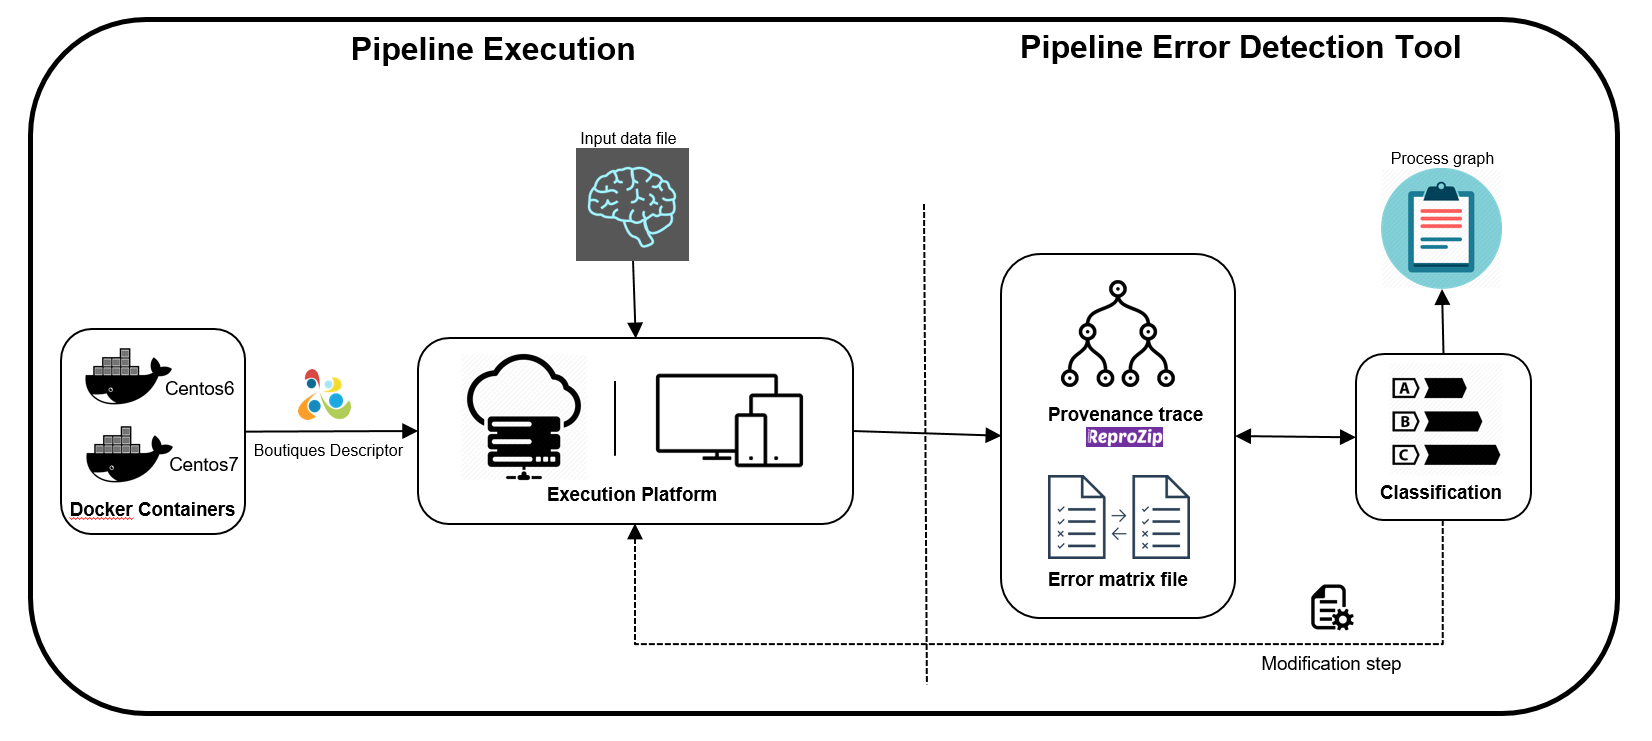
\includegraphics[scale=0.9]{images/overview.png}
  \caption{An overview of proposed technique.}
  \label{fig:overview}
\end{figure}

Figure~\ref{fig:overview} illustrate an overview of the proposed technique. First, we execute pipelines in a
consistence environments and then the origin of errors in the pipeline is detected through a
classification approach. We will explain each step in detail in the following sections.

\subsection{Measuring differences}



We computed a file difference matrix between files produced for every
subject in every operating system based on MD5 checksums~\cite{md5}
(\url{https://tools.ietf.org/html/rfc1321}) as
in~\cite{Scaria2017}. MD5 is suitable to identify incidental file
differences, although it is not cryptographically secure. Files
produced only in some subjects or in some operating systems were left out.

We quantified the error in the image files using the Dice coefficient and normalized root mean square error (NRMSE) computed as follows:
\begin{center}
\begin{equation}
RMSE = {\sqrt {\frac{1} {n}{\sum\limits_{t = 1}^n {(\hat{y}_{t} - {y}_{t} } })^{2} } }
\end{equation}
\end{center}

\begin{center}
\begin{equation}
NRMSE = {\frac{RMSE} {y_{max} - y_{min}}}
\end{equation}
\end{center}

\subsection{Pipeline analysis: Characterizing errors}

Once errors between conditions are quantified, we automatically
identify the steps in the pipeline responsible for such differences.
We use the \reprozip tool~\cite{reprozip} to record: (1) the tree of
processes executed by the pipeline and (2) the list of files read and
written by each process. This information is collected by system call
interceptions, through the \texttt{ptrace} Unix system call, and
stored in a \texttt{SQLite} database. The database stores information
on all the processes which are created by the \texttt{clone()} or
\texttt{fork()} system calls. It also records the files opened by each
process (in read, write or execution mode), including the result files
and the temporary files.

We reconstruct the tree of processes starting from the first process
created by the pipeline and identifying its child processes as the ones
that were created through \texttt{clone()} or \texttt{fork()}. We
create a process graph from this tree by adding edges corresponding to
file dependencies between processes. A file dependency is defined
between processes A and B if a file written by A is read by
B. Figure~\ref{fig:simple_script} shows an example of a process graph
constructed at this stage.

\medskip
\noindent
\begin{minipage}[]{.5\linewidth}
  \centering
  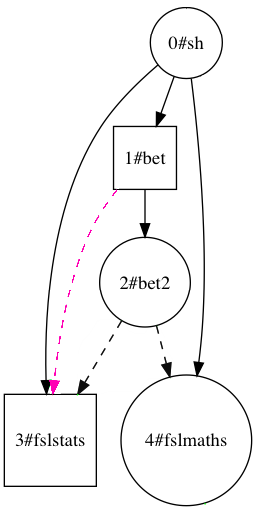
\includegraphics[scale=0.2,width=.4\linewidth]{images/simple_graph}
%  \captionof{figure}{This is a figure caption.} \label{myfig1}
\end{minipage}
\begin{minipage}[]{.3\linewidth}
\small\captionof{algorithm}{sample script of a process graph}\label{sample_script}
{\scriptsize
\begin{verbatim}
#!/bin/bash
if [ # !=1 ]
then
    echo "usage: 0 <inputimage.nii.gz>"
    exit 1
fi
input_image=$1
bet_output="$(basename ${input_image} .nii.gz)_brain.nii.gz"
bet_output_binarized="$(basename ${input_image} .nii.gz)_brain_bin.nii.gz"

bet ${input_image} ${bet_output} > bet_temp.out
echo "Voxels / Volume in brain mask:"
fslstats ${bet_output} -V
fslmaths ${bet_output} ${bet_output_binarized}
echo "Voxels / Volum in binarized brain mask:"
\rm bet_temp.out
\end{verbatim}
}
\end{minipage}
\captionof{figure}{Process graph constructed from an example brain extraction
    script. Every node in the graph is labeled using (1) a process id
    created by our reconstruction, (2) the name of the executable run
    by the process. Processes that read or write temporary files are
    represented with squares; other ones with circles. Plain edges
    represent the process tree (\texttt{fork()} or \texttt{clone()}
    system calls). Dashed edges represent file dependencies: temporary
    files are in yellow and result files are in green.} \label{fig:simple_script}
\medskip

A different process graph may be produced for every subject in every
execution condition. Among our dataset, we identified 4 types of
subjects with different numbers of T1w and T2w images. We verified
that the process graphs were identical for all subjects of the same
type, for all execution conditions \todo{Check that}. The remainder of
the analysis is done separately for each subject type.

Cycles may be present in the process graph in case a file was written 
by more than one process. We remove such cycles by removing file edges 
between processes A and B when A's process creation timestamp is 
posterior to B's or when A=B. Indeed, such edges cannot happen in 
practice unless A and B were running concurrently, which we assume is 
not the case (we also checked that on the workflow we tested). 

\paragraph{} In the next step, we classify the processes into three 
categories based on the process graph and the error matrix file 
mentioned in the previous Section:
\begin{enumerate}
\item Processes that read files that do not have errors and write files that do not 
have errors are \emph{transparent} (Figure~\ref{fig:processes}.a).
\item Processes that read files 
that do not have any error but write files that have errors 
\emph{create} errors in the pipeline (Figure~\ref{fig:processes}.b).
\item Processes that read files 
that have errors and write files that do not have errors \emph{remove} 
errors from the pipeline (Figure~\ref{fig:processes}.c).
\item Processes that read files that have errors and write files that also have errors are 
\emph{unknown} (Figure~\ref{fig:processes}.d).
\end{enumerate}

\begin{figure}[H]%\centering
    \begin{subfigure}{0.15\textwidth}
        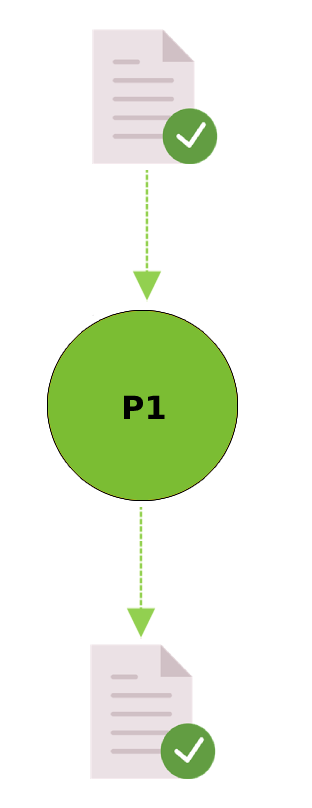
\includegraphics[scale=0.35]{images/green.png}
        \caption{Transparent}
        \label{fig:green}
    \end{subfigure}
\hfill%\hfil
    \begin{subfigure}{0.15\textwidth}
    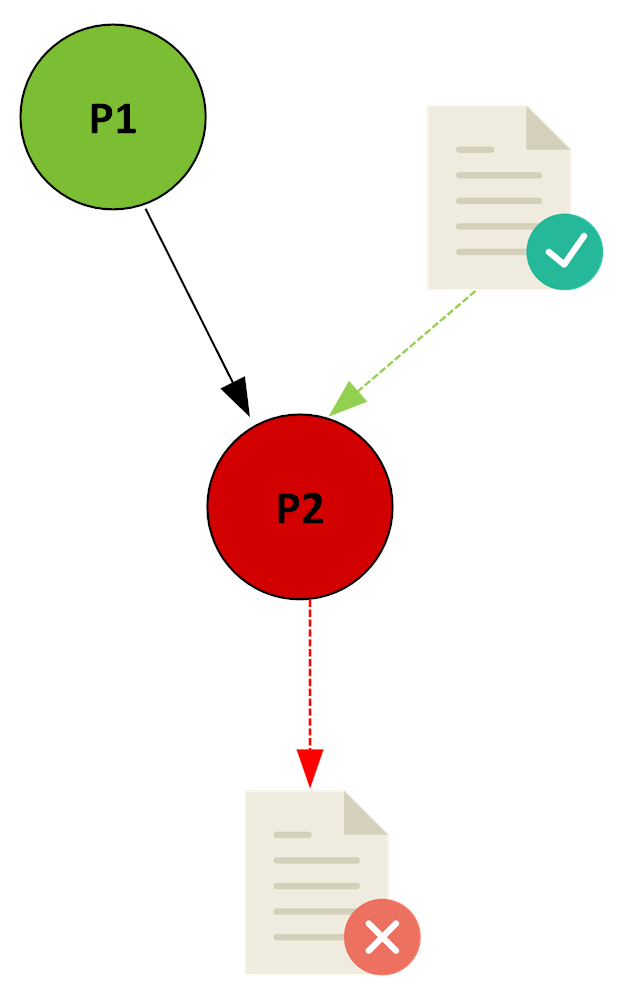
\includegraphics[scale=0.35]{images/red.png}
    \caption{Creates error}
    \label{fig:red}
\end{subfigure}
\hfill%\hfil
    \begin{subfigure}{0.15\textwidth}
    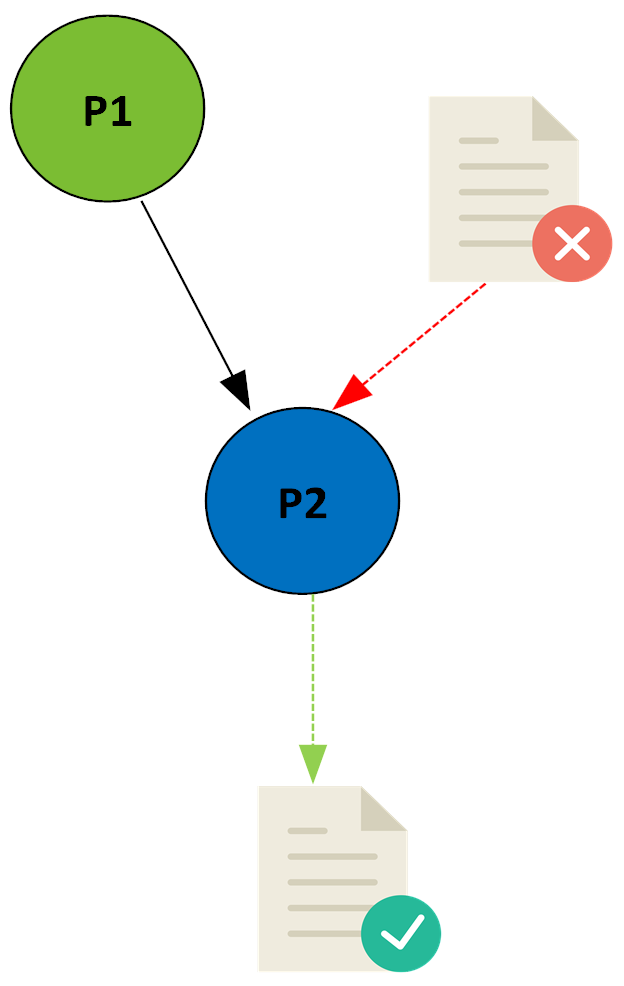
\includegraphics[scale=0.35]{images/blue.png}
    \caption{Removes error}
    \label{fig:blue}
\end{subfigure}
\hfill%\hfil
    \begin{subfigure}{0.15\textwidth}
    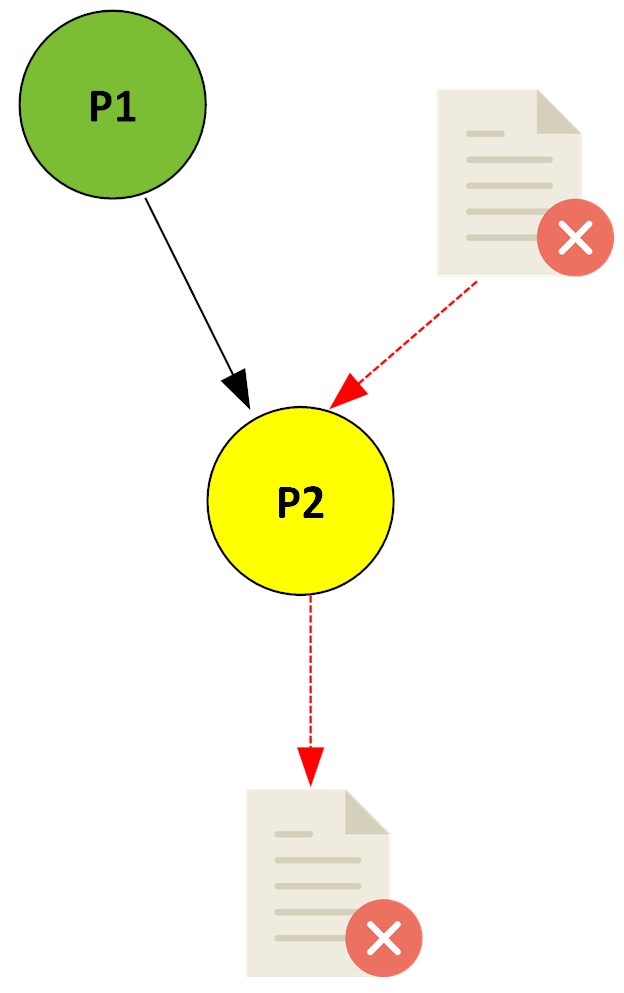
\includegraphics[scale=0.35]{images/yellow.png}
    \caption{Unknown}
    \label{fig:yellow}
\end{subfigure}
    \caption{Different type of classified process based on the input/output files.
  Dashed edges refer to the file dependencies between processes A and B if a file written bu A is read bu B.
  Solid black edges refer ti the relationship between parent and child processes.}
    \label{fig:processes}
\end{figure}

\paragraph{Challenge1:} The classification of processes that read or write temporary files is 
uncertain when these files are deleted during the execution. To address 
this issue, we replace every process P that writes temporary files with 
a modification of P that first calls P and then backs up all its output 
files to a read-only directory. This replacement is done by modifying 
the Unix PATH variable to point to a directory containing the modified
versions of the processes. This solution does not cover the temporary files
that are removed by P itself; this is not a problem since these files do not
play any role in the subsequent steps of the pipeline, by definition.

\paragraph{Challenge2:} Files written by multiple processes also lead to unknown classification 
labels. To address this issue for a file F written by processes in 
\textbf{P} = \{$P_{1}$, \ldots $P_{n}$\}, we (1) check that processes 
in \textbf{P} do not write concurrently to F, (2) we establish an order 
on \textbf{P} based on the creation timestamp of the processes, (3) we 
replace ever process $P_{i}$ in \textbf{P} by a wrapper that first 
calls $P_{i}$ and then backs up F to a read-only directory. Thus, 
multiple versions of F are saved and used in the analysis.

\paragraph{Challenge3:} Another challenge is to classify processes that read files that have
errors and write files that also have errors. In such situations, it
is not possible to determine from the pipeline results whether
the process created errors, removed some errors, or was
transparent. We label such processes \emph{unknown}. To address this issue, we developed an iterative approach that consists of the following steps:
\begin{enumerate}
  \item Run the pipeline in conditions 1 and 2; classify the
    processes as \emph{transparent}, \emph{create errors},
    \emph{remove errors} or \emph{unknown}.
  \item If there are \emph{unknown} processes then: replace each process P that create errors by a process Q that
    copies the results produced by process P in condition 1 to the pipeline output in condition 2.
  \item Repeat steps 1 and 2 until there is no \emph{unknown} process left.
\end{enumerate}

The replacement of process P at step 2 is done by replacing P
with a custom script produced by step 1. This custom script
copies the results obtained in condition 1 if it is invoked with the
arguments of a process that created errors, and calls P's original
executable otherwise. The replacement is done through the PATH variable, as before.
This algorithm converges to a process graph without any \emph{unknown} process after
a finite number of iterations.

\begin{figure}[H]
\centering
  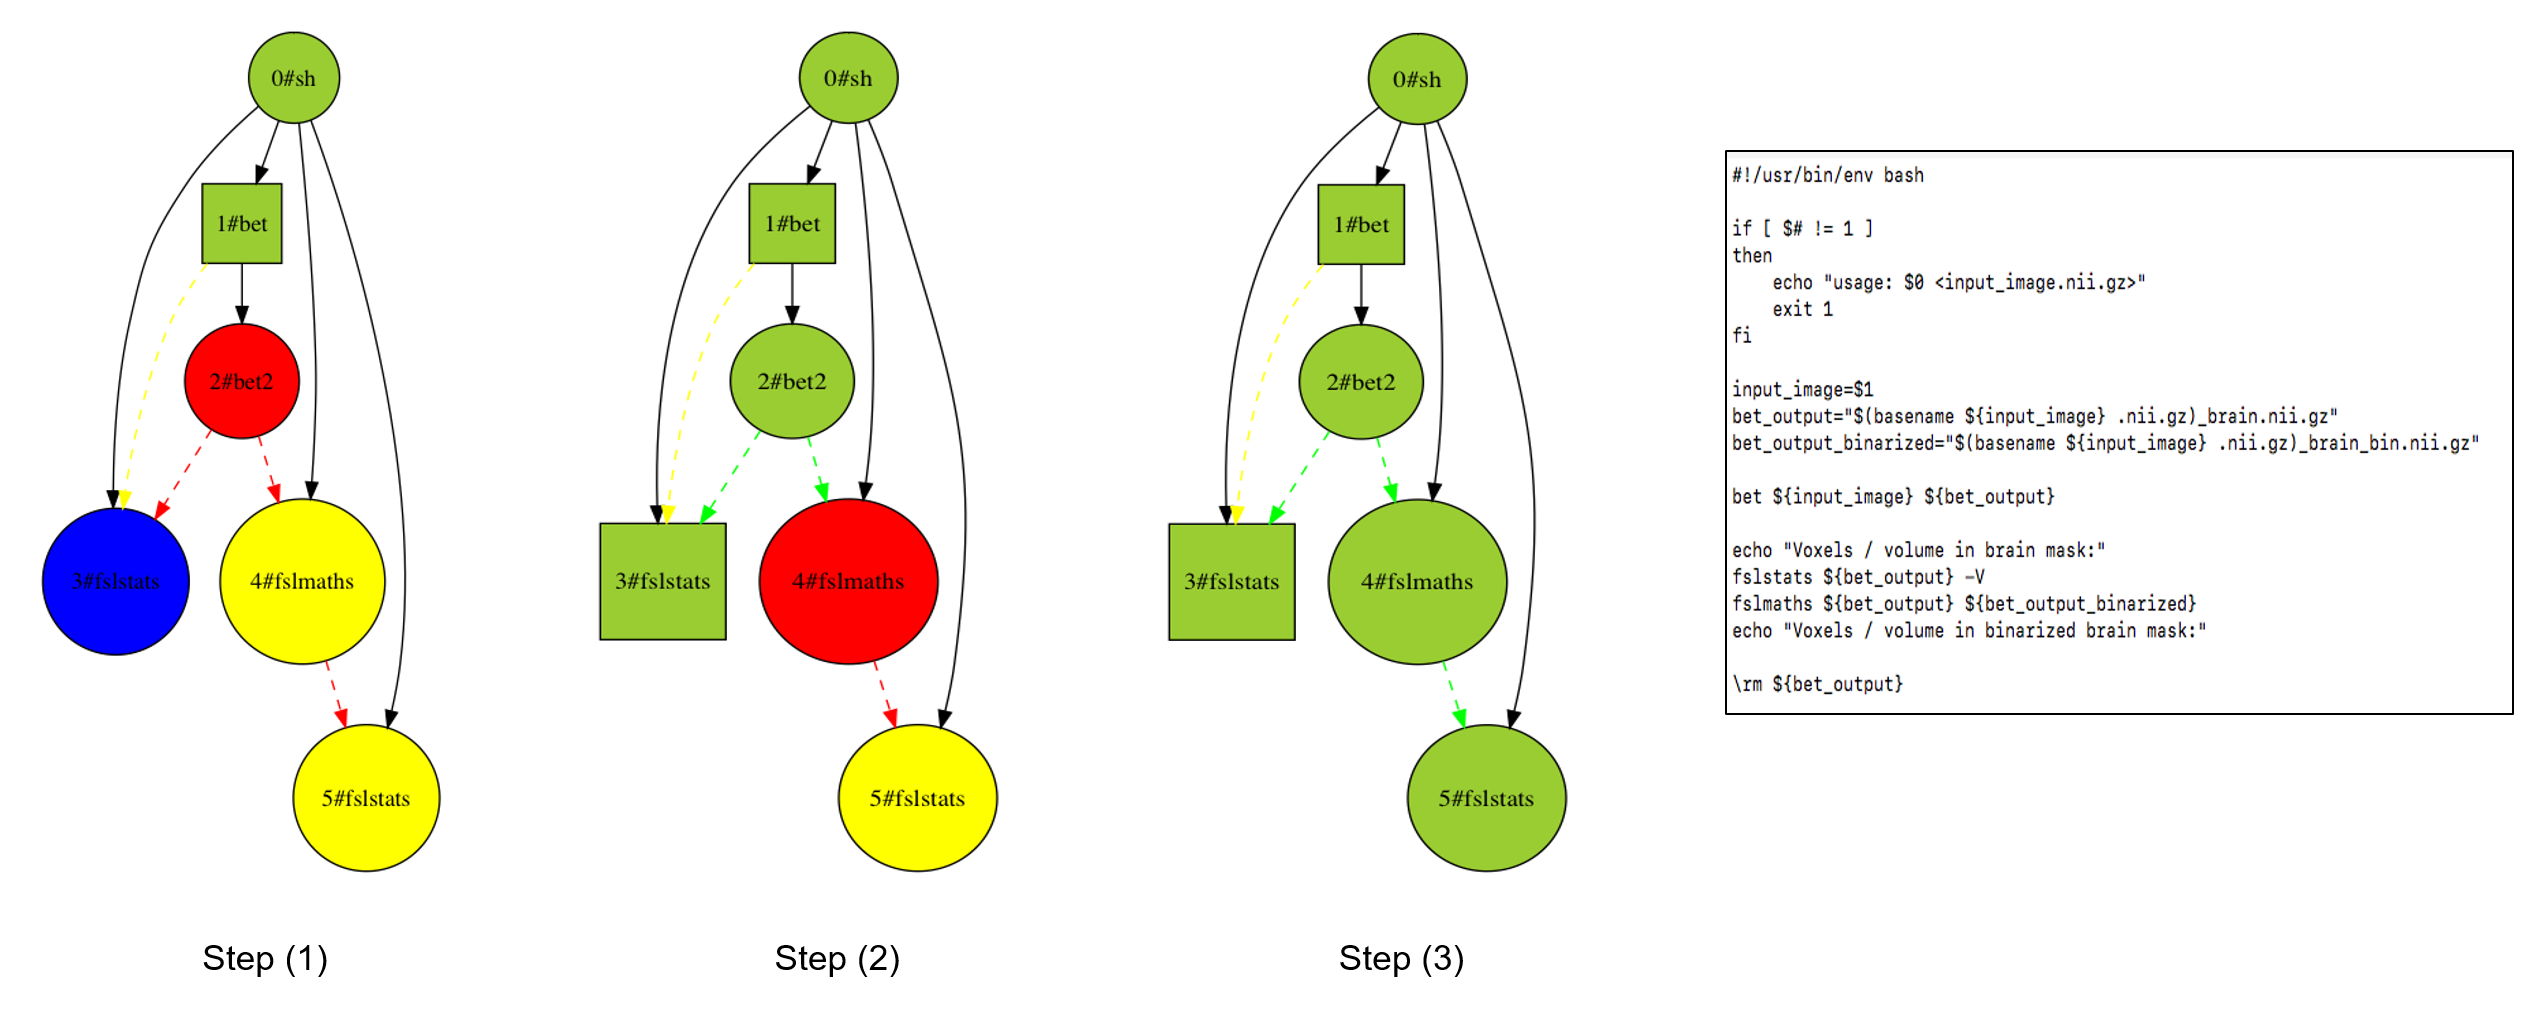
\includegraphics[scale=0.5]{images/iterative_modif}
  \caption{iteration of proposed modification.}
  \label{fig:iterations}
\end{figure}

Figure~\ref{fig:iterations} illustrates our iterative classification 
process for the example in Figure~\ref{fig:graph-example}. At every 
step, processes that created errors are shown in red, processes that 
removed errors are in blue, processes that propagated errors are in 
yellow, and other processes (transparent processes) are in green. As in 
Figure~\ref{fig:graph-example}, plain black edges represent the process 
tree and dashed edges represent file dependencies: green edges 
represent files with no errors, while red edges represent files with 
errors. Temporary files are not represented because they have been 
backed up as previously described.

The three steps in Figure~\ref{fig:iterations} correspond to the 
iterations of the classification algorithm At step one \texttt{2\#bet2} 
is classified as error creator (red) as it produced files with errors 
from files without error. \texttt{3\#fslstats} is classified as error 
remover (blue) as it produced files without errors from files with 
errors. \texttt{4\#fslmaths} and \texttt{5\#fslstats} are classified as 
unknown (yellow) as they produce files with errors from files with errors.

At step 2, the files produced by \texttt{2\#bet2} in the tested 
condition are replaced with the files produced by \texttt{2\#bet2} in 
the other condition. \texttt{3\#fslstats} is now classified as transparent, \texttt{4\#fslmaths} is now classified
as error creator and \texttt{5\#fslstats} is still unknown.

 At step 3, the files produced by \texttt{4\#fslmaths} in the tested 
 condition are replaced with the files produced by \texttt{4\#fslmaths} 
 in the other condition. \texttt{5\#fslstats} is now transparent.
 
 As a result of those 3 steps, the final process classification is: 
 \texttt{2\#bet2} and \texttt{4\#fslmath} are error creators (red), 
 \texttt{3\#fslstats} is error remover (blue) and the other processes 
 are transparent.

The process graphs of real pipelines are much larger than the one in 
Figure~\ref{fig:iterations}. To represent such large graphs, we 
summarize them by (1) building subgraphs for every interesting node 
(e.g. red and blue nodes with their children) (2) building connected components 
in the absence of interesting nodes for the remaining nodes in the process graph. 
Each node in the summarized graph represent either a shrinked interesting subgraph or 
connected component and edges represent any connection between two shrinked nodes.

\section{Results}

Show lists of packages used with version. Focus on important
differences (e.g.: python interpreter, gcc if relevant) and explain
why these packages are important.

Show results of the comparison.

\subsection{Inter-OS differences}


\paragraph{Binary differences}


Among the 117 data files produced by PreFreeSurfer, 21 did not have any error for any subject, 92 had errors 
for all subjects and 4 had errors for 3 subjects only. 

In a previous study~\cite{Scaria2017}, we showed that
pre-processing pipelines of the Human Connectome
Project~\cite{Glasser2013} were sensitive to operating system
variation (see Figure \ref{fig:1}).
\begin{figure}[H]
%  \includegraphics{brain\_classification}
  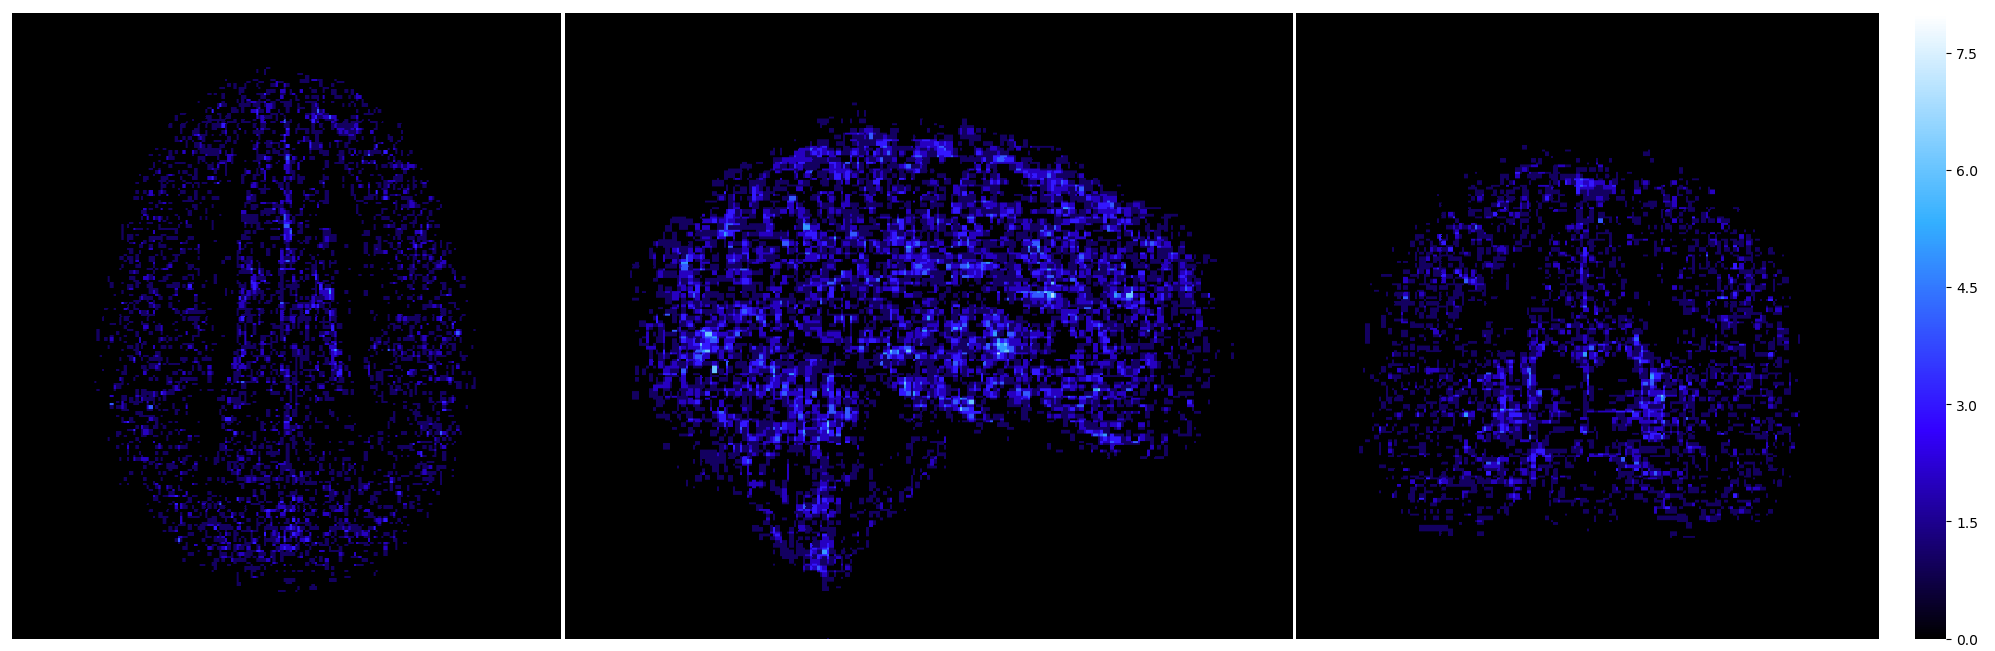
\includegraphics[width=0.5\textwidth, height=6cm]{images/brain_classification.png}
  \caption{Tissue classification produced by the HCP pre-processing
    pipelines on subject 105216 (CentOS 6 vs CentOS 7).}
  \label{fig:1}
\end{figure}

\begin{figure}[H]
\centering
  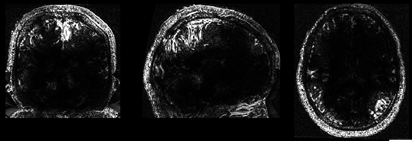
\includegraphics[scale=0.8]{images/fnirt_result.png}
  \caption{Differences between FNIRT results (T2w\_acpc\_to\_MNI\_nonli.nii.gz), subject 104820 (centos6 vs. centos7).}
  \label{fig:fnirt_result}
\end{figure}

\paragraph{}
Two types of differences can occur in the subjects due to the differences in the operating systems. 
One is inter-OS difference caused by the operating system library updates and the other type,
 intra-OS differences occurs as a result of the pseudo-random processes used in the pipelines.
 An example of a pseudo-random process function is, a random number generator that would get initialized 
using a seed state. the proposed method can be used to identify both kind of differences. 
The files that are common to all the subjects only are taken into consideration for comparison. The first step
 is identification of files with differences in their checksums. This is identified using the checksums that are
 recorded after the processing. Intra-OS differences are identified using the run-number added as the suffix for
 the conditions. For example, the two batches of subjects processed under the same condition (CentOS6) are stored 
as run-1 and run-2. The files belonging to the subjects stored under the above mentioned conditions are treated as intra-OS runs.



\subsection{Pipeline analysis}

Figure \ref{fig:summarized-graph} shows the annotated provenance graph of the
PreFreeSurfer pipeline executed on CentOS6 and CentOS7.
Each node in the graph represent an executed process in the pipeline.
Processes that created errors are shown in red, processes that removed errors
are in blue, and other processes are in green.  Squares denote
processes for which the classification is uncertain, due to temporary
files that were removed during the execution. Black edges link
sub-processes to their parents while dashed edges denote file
dependencies between processes (green edges: files with no errors; red
edges: files with errors; yellow edges: temporary files).

The processes that introduce errors in PreFreeSurfer are: linear
registration with “\emph{FLIRT}” (8 occurrences, in ACPC Alignment,
BrainExtraction, DistortionCorrection, AtlasRegistration), non-linear
registration with “\emph{FNIRT}” (3 occurrences, in BrainExtraction
and AltasRegistration), image warping with “\emph{new\_invwarp}” (3
occurrences, in BrainExtraction and AtlasRegistration).  In addition,
errors were observed in image mean and standard-deviation computations
with “\emph{fslstats}” (3 occurrences in BiasFieldCorrection), and in
masked image extrapolation with “\emph{fslmaths}” (1 occurrence, in
BiasFieldCorrection).  Besides, transformation format conversion with
“\emph{convertwarp}” (2 occurrences, in DistortionCorrection) was able
to remove errors.

\todo{Check if a given file is written by only one process (add a safeguard in your code).}


\begin{figure}[H]
\centering
  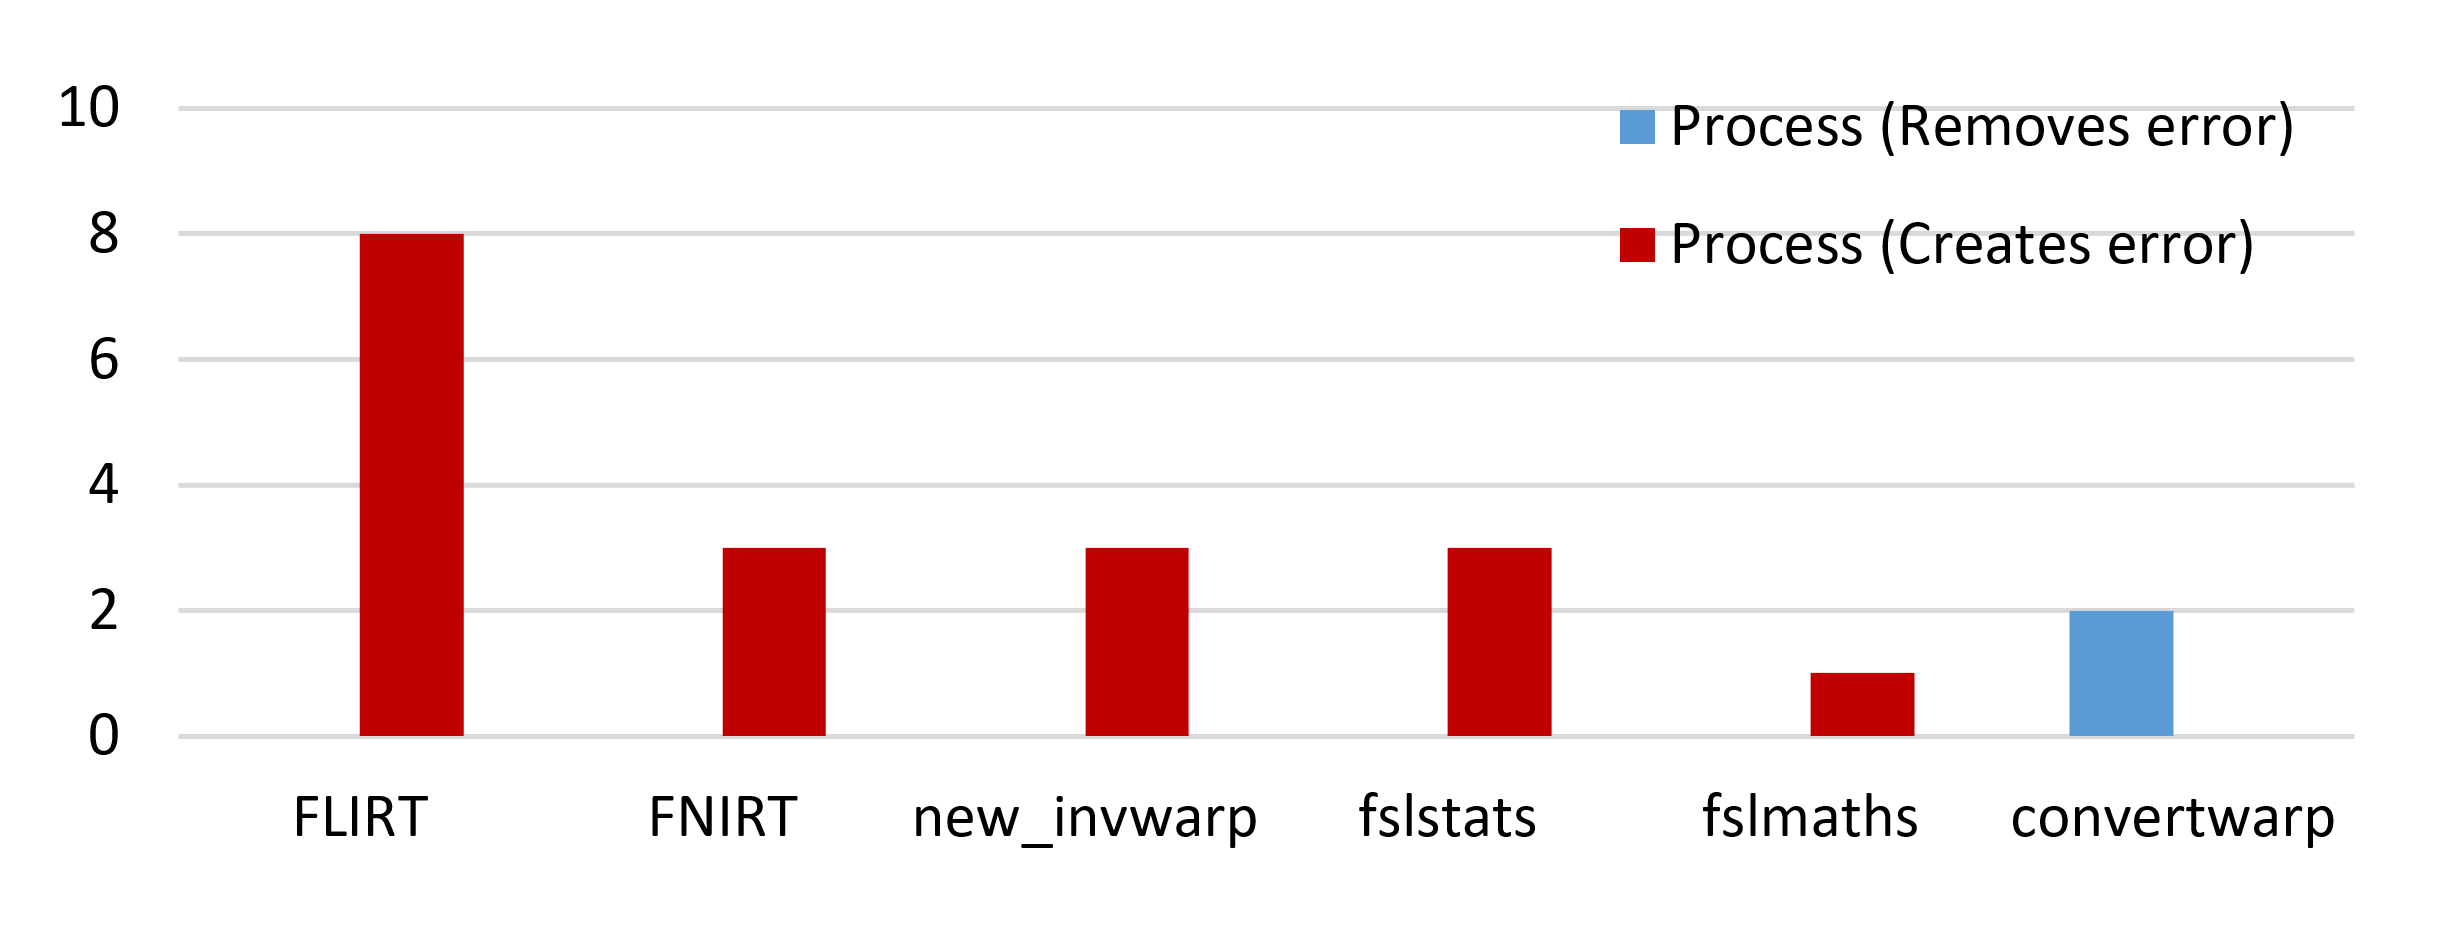
\includegraphics[scale=0.3]{images/pfs_chart.png}
  \caption{Number of occurrences of errors in PreFreeSurfer, red and blue bars 
indicate the processes which create and remove errors respectively.}
  \label{fig:pfs_chart}
\end{figure}

\begin{figure}[H]
\centering
  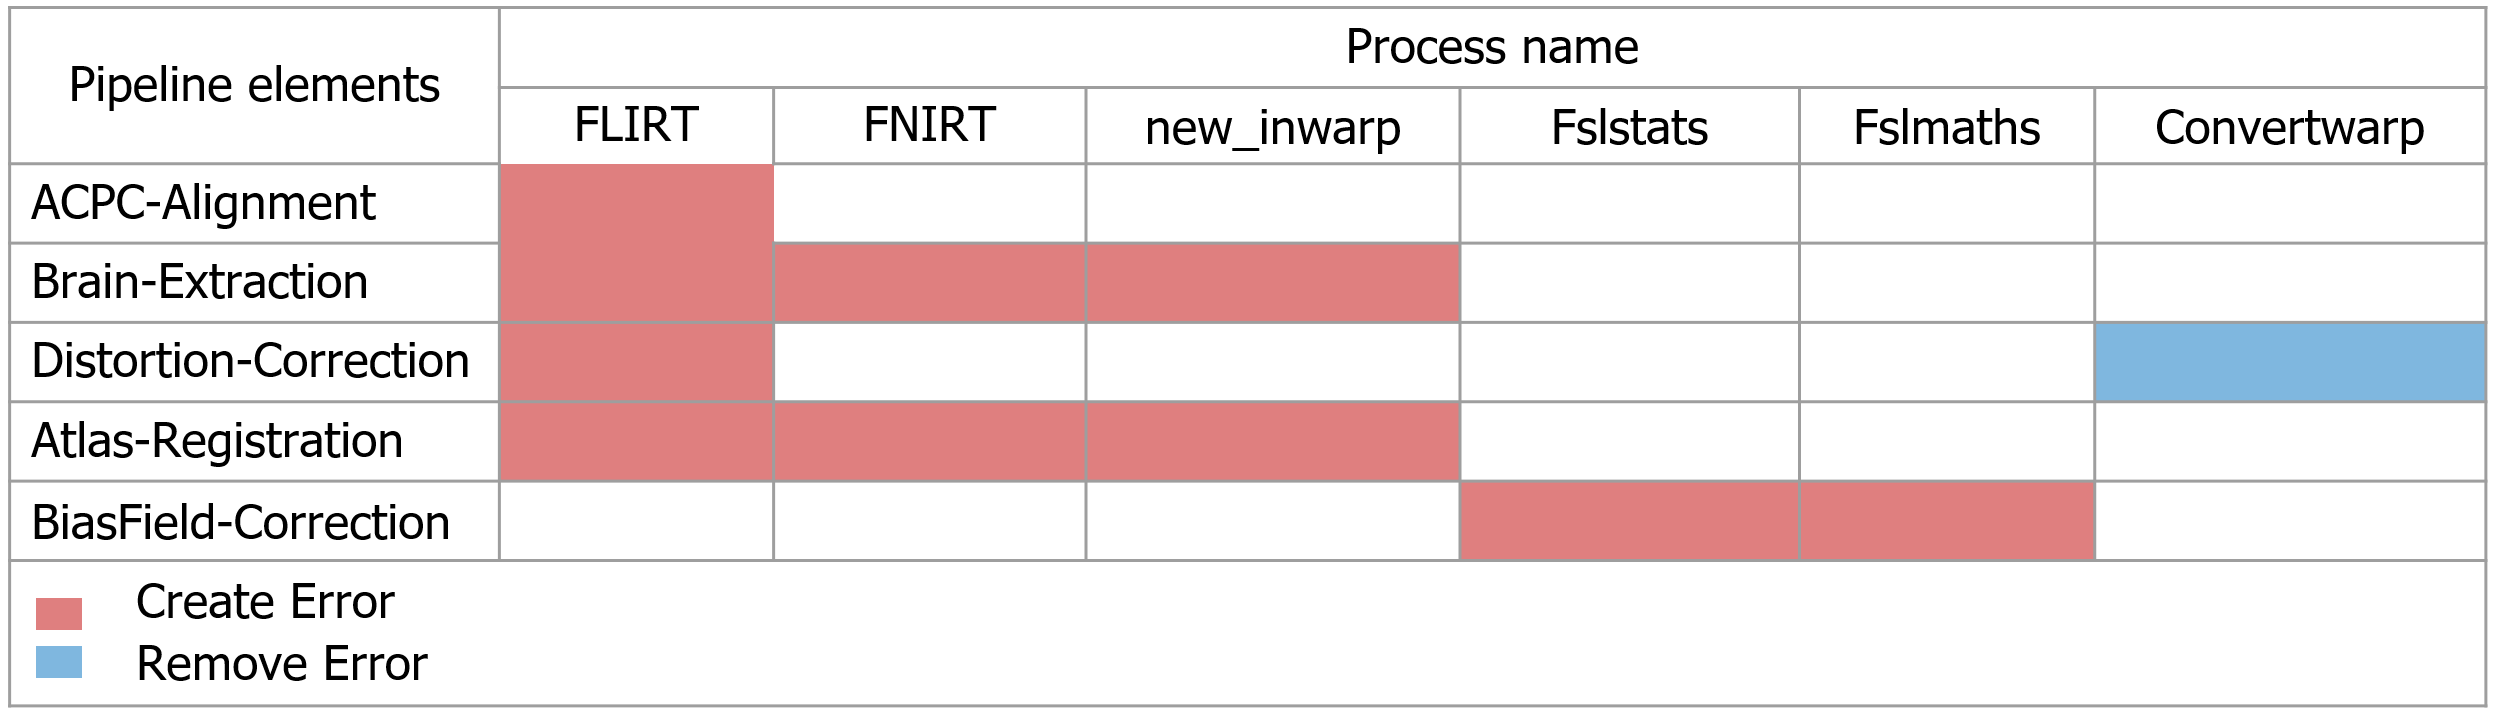
\includegraphics[scale=0.5]{images/pfs_table.png}
  \caption{Process name along with the pipeline elements that inbtroduce errors.}
  \label{fig:pfs_table}
\end{figure}

The processes that introduce errors in FreeSurfer are shown on Figure~\ref{fig:fs_error_table}.
Also, processes that remove errors in FreeSurfer represented on Figure~\ref{fig:fs_remove_table}.
\begin{figure}[H]
\centering
  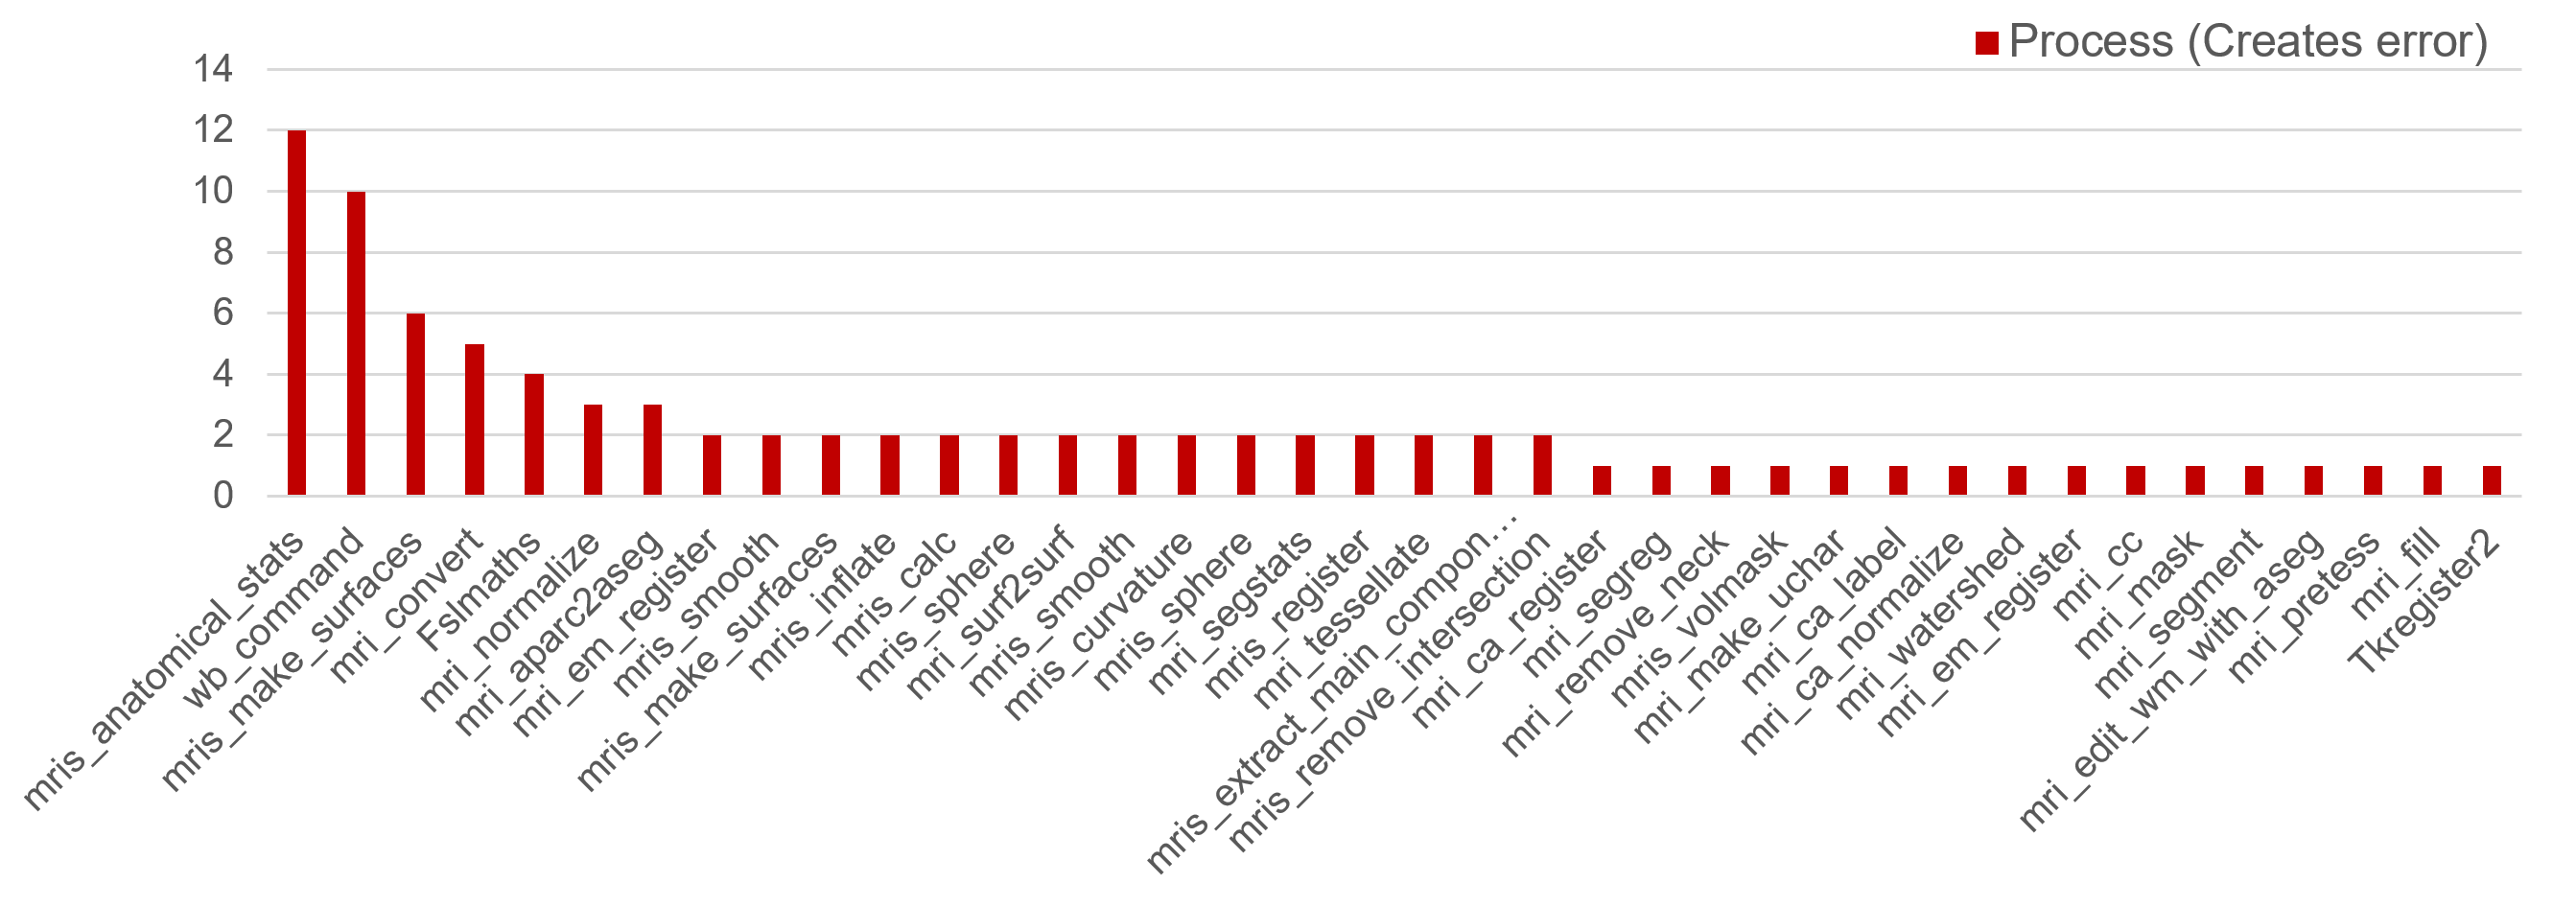
\includegraphics[scale=0.5]{images/fs_error_table.png}
  \caption{Number of occurrences of errors in FreeSurfer pipeline, subject 103818, 
indicate the processes that create errors.}
  \label{fig:fs_error_table}
\end{figure}

\begin{figure}[H]
\centering
  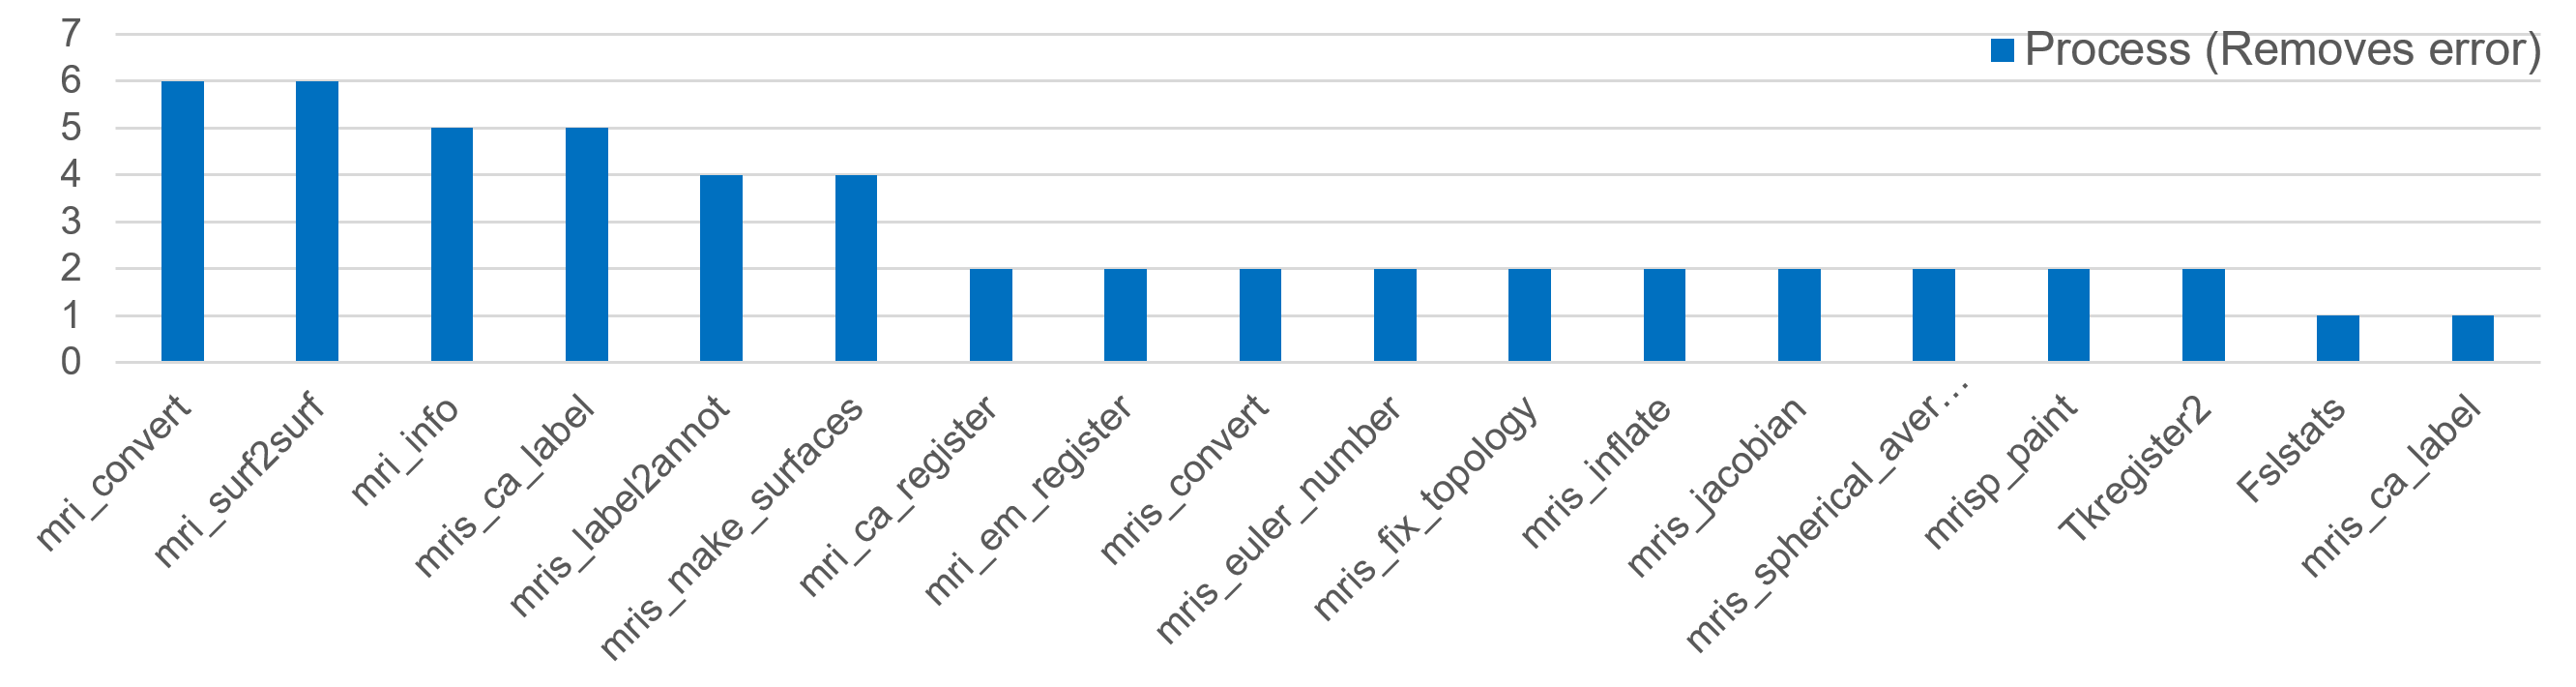
\includegraphics[scale=0.5]{images/fs_remove_table.png}
  \caption{Number of occurrences of errors in FreeSurfer pipeline, subject 103818, 
indicate the processes that remove errors.}
  \label{fig:fs_remove_table}
\end{figure}


\section{Discussion}

pipeline amplify small numerical differences, they are numerically unstable.
Furthermore, math libraries evolve over time, leading to different numerical errors.
we listed some of the irreproducibility causes of the pipelines as we mentioned
in the previous section overally along with exact command arguments.

\begin{itemize}
\item FSLSTATS: Calculate statistics on an image (mean, standard deviation and etc.)
    \begin{lstlisting}[language=bash, basicstyle=\tiny]
STD=`${FSLDIR}/bin/fslstats $WD/T1wmulT2w_brain_norm_modulate.nii.gz -S` 
MEAN=`${FSLDIR}/bin/fslstats $WD/T1wmulT2w_brain_norm_modulate.nii.gz -M` 
    \end{lstlisting}
\item FSLMATH: Create and apply a binary mask to filling of holes to remove  any non-grey/white tissue
using a threshold created by FSLSTATS at Mean.
    \begin{lstlisting}[language=bash, basicstyle=\tiny]
{FSLDIR}/bin/fslmaths $WD/T1wmulT2w_brain_norm_modulate -thr $Lower -bin -ero -mul 255 
                      $WD/T1wmulT2w_brain_norm_modulate_mask ${CARET7DIR}/wb_command -volume-remove-islands 
                      $WD/T1wmulT2w_brain_norm_modulate_mask.nii.gz $WD/T1wmulT2w_brain_norm_modulate_mask.nii.gz
    \end{lstlisting}

\item FLIRT: Register cropped image to MNI152 (12 DOF)
    \begin{lstlisting}[language=bash, basicstyle=\tiny]
{FSLDIR}/bin/flirt -interp spline -in "$WD"/robustroi.nii.gz -ref "$Reference"
                   -omat "$WD"/roi2std.mat -out "$WD"/acpc_final.nii.gz
                   -searchrx -30 30 -searchry -30 30 -searchrz -30 30

{FSLDIR}/bin/flirt -interp spline -dof 6 -in ${WD}/Magnitude_warpped${TXw}
                    -ref ${TXwImage} -out ${WD}/Magnitude_warpped${TXw}2${TXwImageBasename}
                    -omat ${WD}/Fieldmap2${TXwImageBasename}.mat
                    -searchrx -30 30 -searchry -30 30 -searchrz -30 30
    \end{lstlisting}

\item FNIRT: non-linear registration to MNI
    \begin{lstlisting}[language=bash, basicstyle=\tiny]
{FSLDIR}/bin/fnirt --in=${T1wRestore} --ref=${Reference2mm} --aff=${WD}/xfms/acpc2MNILinear.mat
                   --refmask=${Reference2mmMask} --fout=${OutputTransform}
                   --jout=${WD}/xfms/NonlinearRegJacobians.nii.gz --refout=${WD}/xfms/IntensityModulatedT1.nii.gz
                   --iout=${WD}/xfms/2mmReg.nii.gz --logout=${WD}/xfms/NonlinearReg.txt
                   --intout=${WD}/xfms/NonlinearIntensities.nii.gz --cout=${WD}/xfms/NonlinearReg.nii.gz --config=${FNIRTConfig}

%~ Register to 2mm reference image (linear then non-linear)
%~ ${FSLDIR}/bin/flirt -interp spline -dof 12 -in "$Input" -ref "$Reference2mm" 
                    %~ -omat "$WD"/roughlin.mat -out "$WD"/"$BaseName"_to_MNI_roughlin.nii.gz -nosearch

%~ ${FSLDIR}/bin/fnirt --in="$Input" --ref="$Reference2mm" --aff="$WD"/roughlin.mat
                    %~ --refmask="$Reference2mmMask" --fout="$WD"/str2standard.nii.gz
                    %~ --jout="$WD"/NonlinearRegJacobians.nii.gz --refout="$WD"/IntensityModulatedT1.nii.gz
                    %~ --iout="$WD"/"$BaseName"_to_MNI_nonlin.nii.gz
                    %~ --logout="$WD"/NonlinearReg.txt --intout="$WD"/NonlinearIntensities.nii.gz
                    %~ --cout="$WD"/NonlinearReg.nii.gz --config="$FNIRTConfig"
    \end{lstlisting}

\item INVWARP \& APPLYWARP: Invert warp and transform dilated brain mask back into native space, and use it to mask input image
    \begin{lstlisting}[language=bash, basicstyle=\tiny]
${FSLDIR}/bin/invwarp --ref="$Reference2mm" -w "$WD"/str2standard.nii.gz -o "$WD"/standard2str.nii.gz
${FSLDIR}/bin/applywarp --rel --interp=nn --in="$ReferenceMask" --ref="$Input" -w "$WD"/standard2str.nii.gz -o "$OutputBrainMask"
    \end{lstlisting}

\item MRIS\_ANATOMICAL\_STATS: Measures a number of anatomical properties
    \begin{lstlisting}[language=bash, basicstyle=\tiny]
mris_anatomical_stats -mgz -cortex ../label/lh.cortex.label -f ../stats/lh.aparc.a2009s.stats -b -a ../label/lh.aparc.a2009s.annot -c ../label/aparc.annot.a2009s.ctab 0050299 lh white
    \end{lstlisting}

\item MRIS\_MAKE\_SURFACES: Generate pial surfaces, first pass, no T2 adjustment. Files created are Xh.pial, Xh.curv.pial, Xh.area.pial, Xh.thickness
    \begin{lstlisting}[language=bash, basicstyle=\tiny]
mris_make_surfaces -variablesigma ${VARIABLESIGMA} -white NOWRITE -aseg aseg.hires -orig white.deformed -filled filled.hires -wm wm.hires -sdir $SubjectDIR -mgz -T1 T1w_hires.norm "$SubjectID" lh
    \end{lstlisting}

\item MRI\_CONVERT:Normalize T1w and T2w images for the benefit of mris\_make\_surfaces

\#Resample the native space binary ROI file into "brainmask" space
    \begin{lstlisting}[language=bash, basicstyle=\tiny]
mri_convert -rl /subA/mri/T1w_hires.nii.gz -rt nearest /subA/mri/filled.mgz /subA/mri/filled.hires.mgz
    \end{lstlisting}

\item MRI\_NORMALIZE: Normalize the white-matter, optionally based on control points.
The input volume is converted into a new volume where white matter image values all range around 110.

\#Uses the norm volume, and creates the brain volume, making use of the aseg and masking with brainmask
    \begin{lstlisting}[language=bash, basicstyle=\tiny]
mri_normalize -aseg aseg.mgz -mask brainmask.mgz norm.mgz brain.mgz
    \end{lstlisting}

\item MRI\_APARC2ASEG:The volumes of the cortical labels will be different than
         reported by mris\_anatomical\_stats because partial volume information
         is lost when mapping the surface to the volume. The values reported by
         mris\_anatomical\_stats will be more accurate than the volumes from the
         aparc+aseg volume.
         
Label the cortex of a subject's segmented volume according to the edited surface labels
    \begin{lstlisting}[language=bash, basicstyle=\tiny]
mri_aparc2aseg --s SUBJ_NUM --volmask
\#slice labeling
mri_aparc2aseg --s ${subject} --labelwm --hypo-as-wm --rip-unknown --volmask --o ${subj_dir}/mri/wmdivided --annot aparc.split
    \end{lstlisting}

\item MRI\_EM\_REGISTER: creates a tranform in lta format
    \begin{lstlisting}[language=bash, basicstyle=\tiny]
mri_em_register -skull -t transforms/talairach.lta nu_noneck.mgz $FREESURFER_HOME/average/RB_all_withskull_2008-03-26.gca transforms/talairach_with_skull.lta
    \end{lstlisting}

\item MRIS\_SMOOTH: Smooths the tessellation of a cortical surface.
    \begin{lstlisting}[language=bash, basicstyle=\tiny]
mris_smooth -nw -seed 1234 ../surf/lh.orig.nofix ../surf/lh.smoothwm.nofix
    \end{lstlisting}

\item MRIS\_INFLATE: inflate cortical surface.
\#The command generates inflated and sulc files.
    \begin{lstlisting}[language=bash, basicstyle=\tiny]
mris_inflate -no-save-sulc surf/lh.smoothwm.nofix surf/lh.inflated.nofix
    \end{lstlisting}

\item MRIS\_CALC: mris\_calc' is a simple calculator that operates on
FreeSurfer curvatures and volumes. In most cases, the calculator functions
with three arguments: two inputs and an <ACTION> linking them.
Some actions, however, operate with only one input <file1>.
In all cases, the first input <file1> is the name of a FreeSurfer curvature overlay (e.g. rh.curv)
or volume file (e.g. orig.mgz). For two inputs, the calculator first assumes
that the second input is a file. If, however, this second input file doesn't exist,
the calculator assumes it refers to a float number, which is then processed according to <ACTION>.Note:
<file1> and <file2> should typically be generated on the same subject.
    \begin{lstlisting}[language=bash, basicstyle=\tiny]

mris_calc -o lh.area.mid lh.area.mid div2
    \end{lstlisting}

\item CONVERTWARP: Forward warp the fieldmap magnitude and register to TXw image (transform phase image as well).
    \begin{lstlisting}[language=bash, basicstyle=\tiny]
${FSLDIR}/bin/convertwarp --relout --rel --ref=${WD}/Magnitude --shiftmap=${WD}/FieldMap_ShiftMap${TXw}.nii.gz 
                          --shiftdir=${UnwarpDir} --out=${WD}/FieldMap_Warp${TXw}.nii.gz
    \end{lstlisting}
\item MRI\_CONVERT:

\item MRI\_SURF2SURF:

\item MRIS\_MAKE\_SURFACE:

\item MRI\_CA\_REGISTER:

\item MRIS\_CONVERT:

\end{itemize}

Mention that this was only possible because the unprocessed data was shared in the first place.
DICOM to Nifti conversion was out of scope and may introduce other issues.

\section{Conclusion}

Our thechnique is able to characterize the stability of a pipeline's components automatically.
The numerical instability in the PreFreesurfer HCP pipeline arises mainly from
linear and non-linear registration processes implemented in FSL FLIRT and FNIRT. 

There are a few ways to impede such instabilities:
\begin{itemize}
\item Use a single operating system
\item Containerize pipelines
\item Increase numerical precision
\item Be stricter on truncation and rounding standards (IEEE 754)
\item Build static executable
\end{itemize}

The results still suffer from small pertubations literally because of the fact that pipeline are not numerically stable.
The preferred solution is to detect and fix numerical instability of the pipeline instead of masking the problem.
These processes need to be reviewed to understand and correct the cause of instabilities. 
In this correction process, accuracy has to be considered in addition to stability.

\item In the future works we aim to measure the impact of such errors
on the specific domain of the neuroscience and how show the significant it is.

\item The purpose of the project is generalizing pipelines to get a reproducible execution 
on every operating system instead of choosing one main OS to.


\section{Acknowledgments}

CBRAIN team. Compute Canada(Calcul Quebec).


\begin{figure}[H]
  \includegraphics[width=\linewidth]{images/summarized_graph}
  \caption{An annotated summarized process graph from the PreFreesurfer pipeline.
Each node in the graph is represented in red, blue or green colors and is labeled 
using the name of the executable run by the interesting process. The close up nodes 
reveal each shrinked subgraph in details.}
  \label{fig:summarized-graph}
\end{figure}

\begin{figure}[H]
  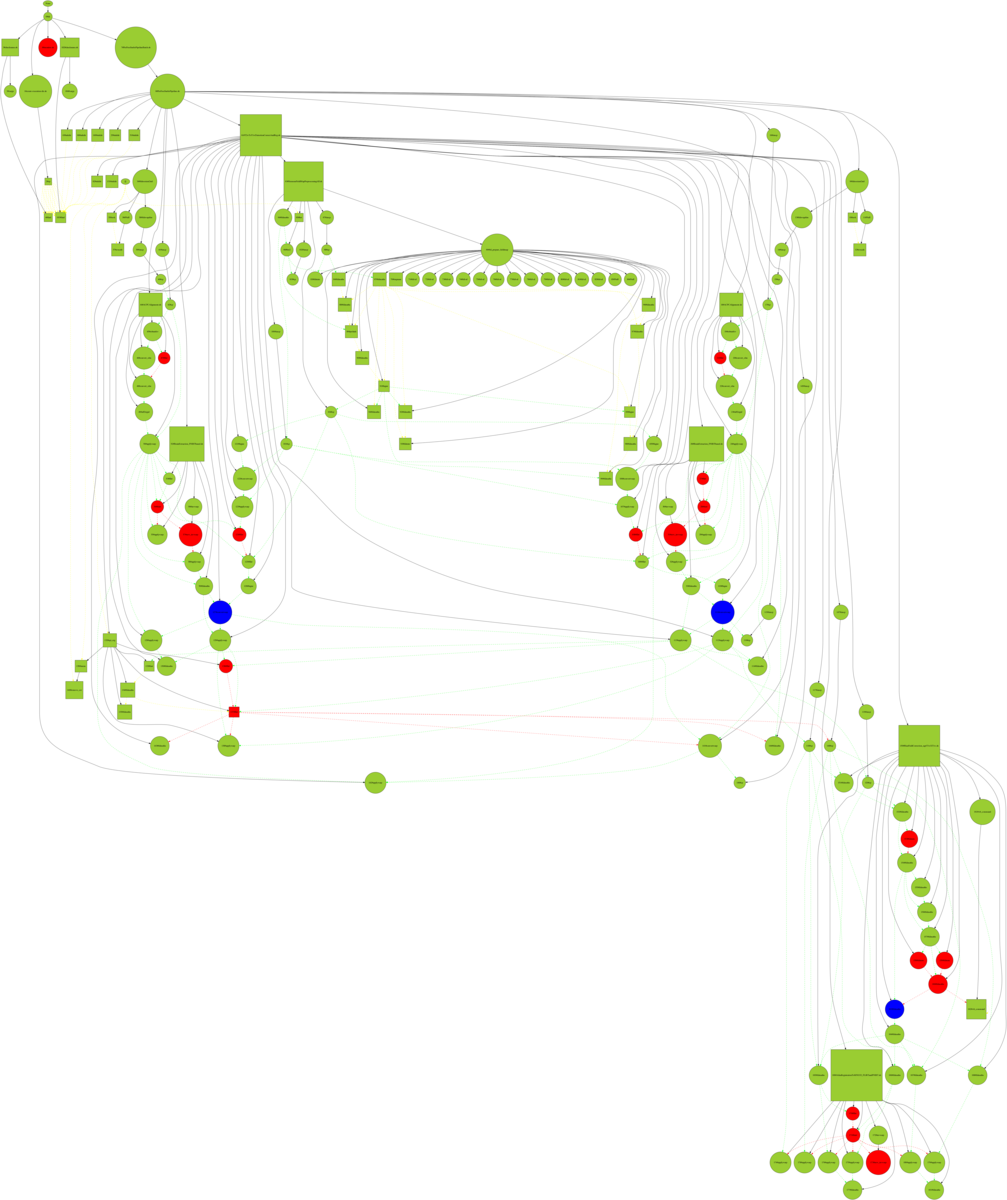
\includegraphics[width=\linewidth]{images/graph}
  \caption{A complete process graph from the PreFreesurfer pipeline.
Full-resolution image available at \url{https://drive.google.com/open?id=174yyn8SuVOUcK5aRVw0bagjDanLD0FLt}.}
  \label{fig:complete-graph}
\end{figure}
\bibliographystyle{plain}
\bibliography{biblio}

\end{document}
